
\documentclass[xcolor={dvipsnames}]{beamer}
\usepackage{amsmath,amsfonts,amssymb,pxfonts,eulervm,xspace}
\usepackage{graphicx}
 \usepackage{multimedia}
\usepackage{media9}
\usepackage{minted}

\graphicspath{{./figures/}}
\usetheme{ccnycrest}


\newenvironment{changemargin}[2]{%
\begin{list}{}{%
\setlength{\topsep}{0pt}%
\setlength{\leftmargin}{#1}%
\setlength{\rightmargin}{#2}%
\setlength{\listparindent}{\parindent}%
\setlength{\itemindent}{\parindent}%
\setlength{\parsep}{\parskip}%
}%
\item[]}{\end{list}}

\begin{document}

\title{ CS102: Selection Structures}
\author{Hannah Aizenman}
\date{haizenm00@ccny.cuny.edu}


\begin{frame}
	\titlepage
\end{frame}

\begin{frame}[fragile]{Hello World}
\begin{columns}
\begin{column}{0.5\textwidth}
\begin{minted}{c++}
#include<iostream>
using namespace std;

int main(){
    cout<<"Hello World!"<<endl;
    return 0;
}
\end{minted}
  \end{column}
  \begin{column}{0.5\textwidth}
	\pause
	\begin{figure}
		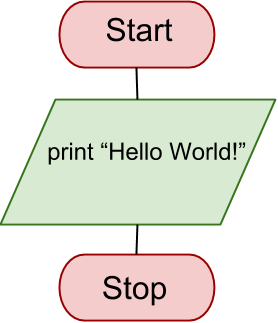
\includegraphics[width=1\textwidth]{hello}
	\end{figure}
  \end{column}
\end{columns}
\end{frame}

\begin{frame}{ What about only sometimes printing "hello"?}
	\pause
	\begin{center}
	\begin{figure}
		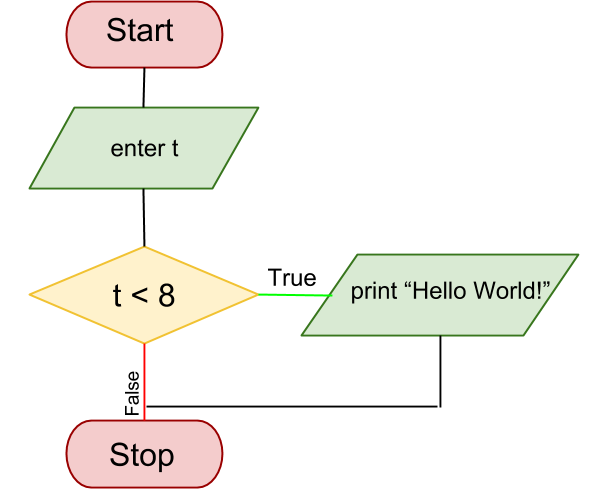
\includegraphics[width=.9\textwidth]{helloif}
	\end{figure}
	\end{center}
\end{frame}

\begin{frame}[fragile]{if statements}
\begin{minted}{c++}
#include<iostream>
using namespace std;

int main(){
    int t;
    cin>>t;
    if (t<8){
        cout<<"Hello World!"<<endl;
    }
    return 0;
}
\end{minted}
\end{frame}

\begin{frame}{How about "hello" or "goodbye" ?}
	\pause
	\begin{center}
	\begin{figure}
		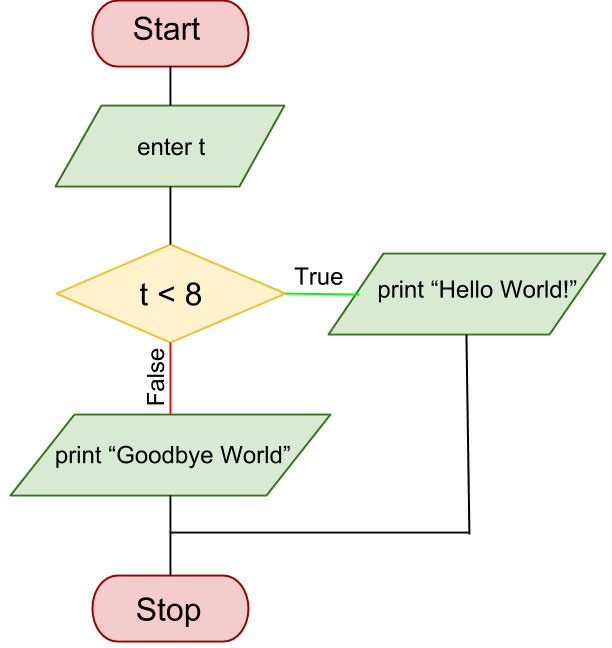
\includegraphics[width=.7\textwidth]{hellogoodbye}
	\end{figure}
	\end{center}
\end{frame}

\begin{frame}[fragile]{if-else statements}
\begin{minted}{c++}
#include<iostream>
using namespace std;

int main(){
    int t;
    cin>>t;
    if (t<8){
        cout<<"Hello World!"<<endl;
    }
    else{
        cout<<"Goodbye World!"<<endl;
    }
    return 0;
}
\end{minted}
\end{frame}

\begin{frame}{"hello", "goodbye", or "nice to meet ya"?}
	\begin{center}	
	\begin{figure}
		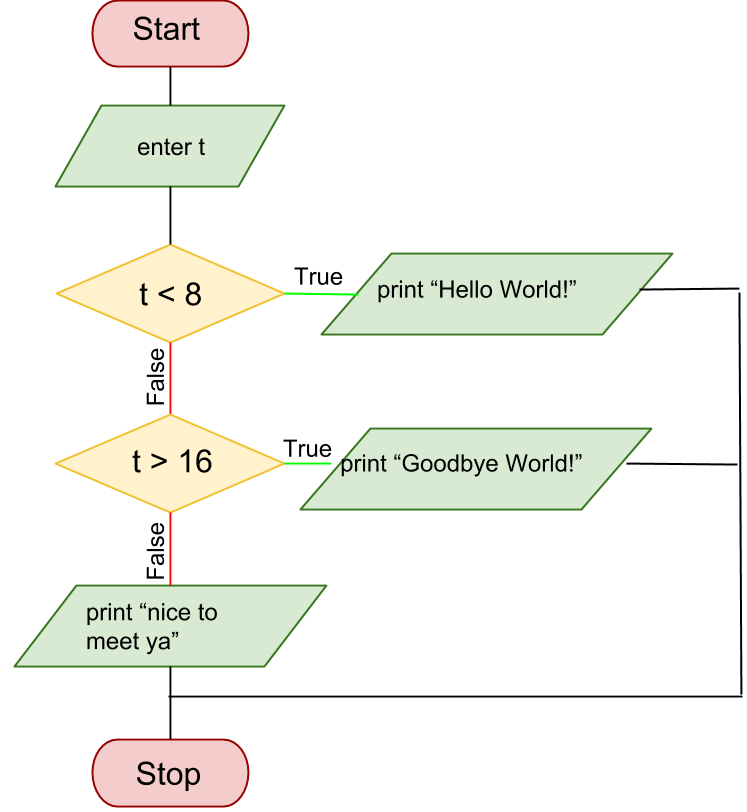
\includegraphics[width=.7\textwidth]{hellogoodbyenice}
	\end{figure}
	\end{center}
\end{frame}

\begin{frame}[fragile]{if else-if else statements}
\begin{minted}{c++}
#include<iostream>
using namespace std;

int main(){
    int t;
    cin>>t;
    if (t<8){
        cout<<"Hello World!"<<endl;
    }
    else if(t>16){
        cout<<"Goodbye World!"<<endl;
    }
    else{
        cout<<"Nice to meet ya!"<<endl;
    }
    return 0;
}
\end{minted}
\end{frame}

\begin{frame}{Nesting}
\begin{center}	
	\begin{figure}
		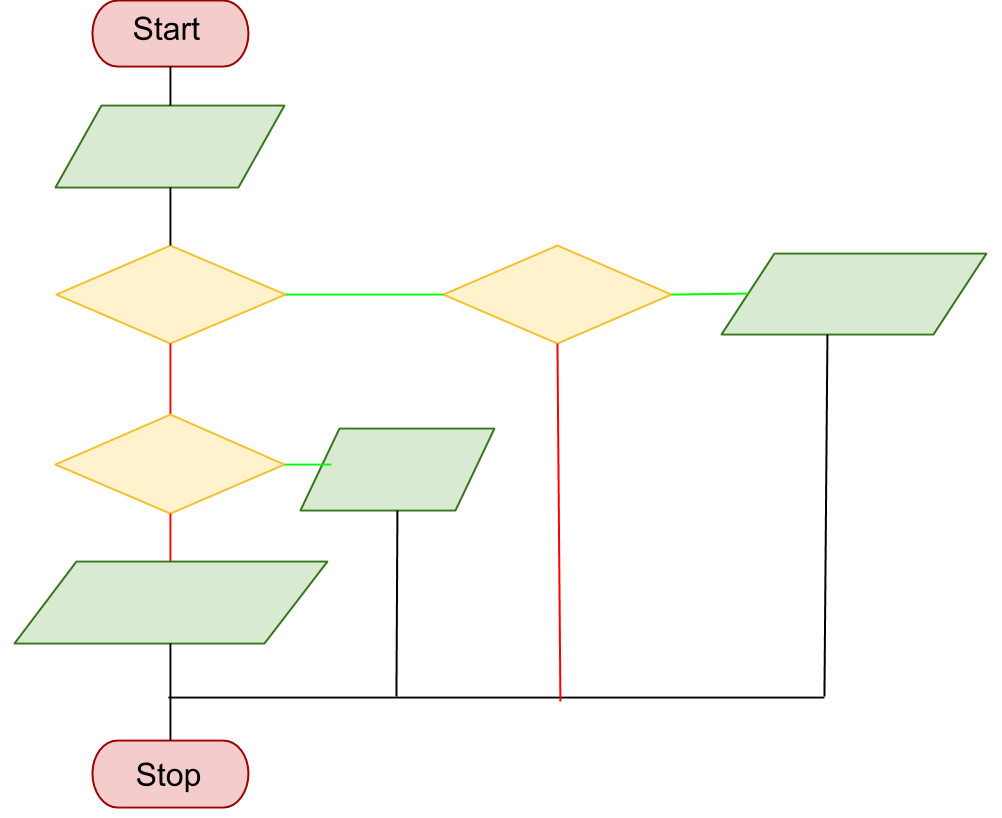
\includegraphics[width=.9\textwidth]{nesting}
	\end{figure}
	\end{center}
\end{frame}

\begin{frame}[fragile]{Nested ifs}
\begin{minted}{c++}
    if (condition){
        if(condition)
            statement;
        }
    }
    else if (condition){
        statement;
    }
    else{
       statement;
    }
\end{minted}
\end{frame}

\begin{frame}{Nesting}
	\begin{itemize}
		\item statements can be nested under ifs or else-ifs
		\item no limit on depth of nesting
		\item can put multiple independent ifs on the same level
		\item indicate nesting using { ...}
	\end{itemize}
\end{frame}

\begin{frame}{Nesting Example}
	\begin{block}{Problem}
		\begin{center}
	 		Find the median of three  integers.
		\end{center}
	\end{block}
	\pause
	\begin{block}{Constraints}
		\begin{itemize}
			\item inputs are unsorted
			\item only allowed to use pairwise comparisons 
			\begin{description}
				\item[no] (a\textgreater b) \&\& (b\textgreater c)
				\item[yes] if (a\textgreater b) \{ if (b\textgreater c)....\}
			\end{description}
		\end{itemize}
	\end{block}
\end{frame}


\begin{frame}{Switch Statement}
\begin{center}	
	\begin{figure}
		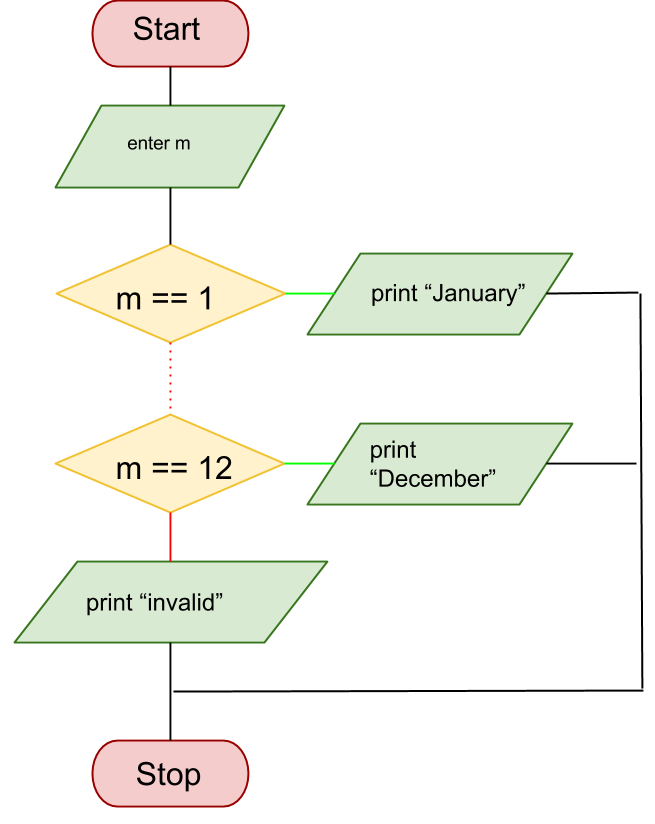
\includegraphics[width=.6\textwidth]{switch}
	\end{figure}
	\end{center}
\end{frame}

\begin{frame}[fragile]{switch statement}
\begin{minted}{c++}
cin>>m;
switch(m){
    case 1: 
        cout<<"January"<<endl; 
        break;
    //cases 2-11
    case 12:
        cout<<"December"<<endl;
        break;
    default:
        cout<<"Invalid"<<endl;
}
\end{minted}
\end{frame}

\begin{frame}{Switch Statement}
\begin{center}	
	\begin{figure}
		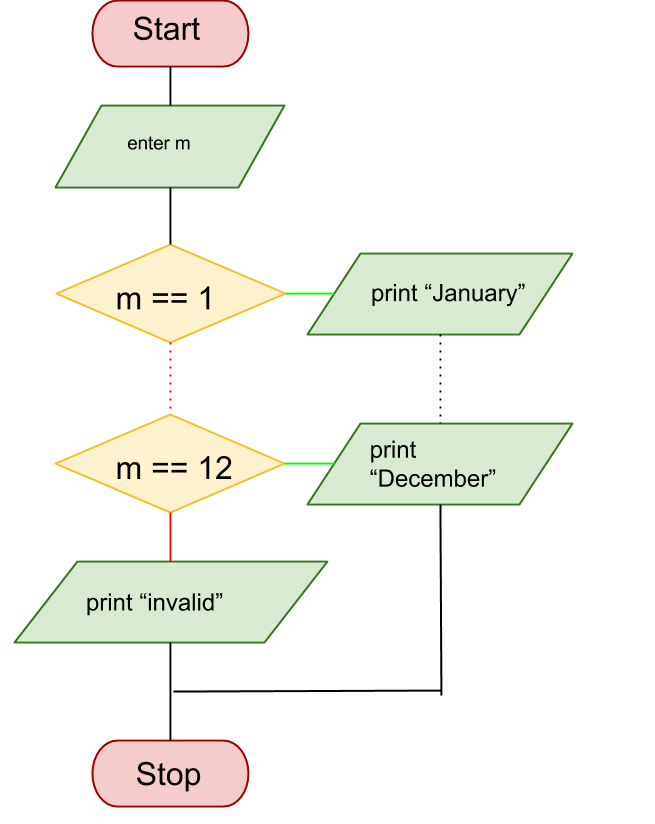
\includegraphics[width=.6\textwidth]{switchnofall}
	\end{figure}
	\end{center}
\end{frame}

\begin{frame}[fragile]{switch statement}
\begin{minted}{c++}
cin>>m;
switch(m){
    case 1: 
        cout<<"January"<<endl; 
    //cases 2-11
    case 12:
        cout<<"December"<<endl;
        break;
    default:
        cout<<"Invalid"<<endl;
}
\end{minted}
\end{frame}

\begin{frame}{Practice}
	\begin{enumerate}
		\item Write a program that takes an integer input and displays the corresponding month name 
		\item Remove the breaks and compare the output
	\end{enumerate}
\end{frame}
\end{document}

